Un pedal de efectos es un dispositivo que se conecta entre un instrumento (normalmente electrófono) y su amplificador encargándose de modificar la señal de entrada y sus características fundamentales como pueden ser timbre, tono y volumen. En este proyecto se pretende estudiar las posibilidades de diseño e implementación de uno de estos pedales, enfocándolo para instrumentos de viento, en concreto el saxofón dado que es el instrumento que yo toco. Generalmente, no es habitual el uso de pedales de efectos en estos instrumentos, ya que se suele buscar mantener el sonido lo más fiel posible al producido de forma natural. No obstante, en multitud de ocasiones se pueden apreciar efectos añadidos en postproducción ya sea digital o analógicamente. Algunos ejemplos son el \emph{reverb} o el \emph{chorus}. Sin embargo, aqui se pretende implementar un efecto de octavador, el cual se describirá posteriormente.

He decidido el combinar este efecto con la implementación en formato de pedal. Este formato se ha hecho muy popular desde su aparición para aplicaciones en tiempo real, debido a que los intérpretes pueden activarlo con el pie pudiendo mantaner las manos en el instrumento. Aunque los intérpretes de instrumentos de viento no están acostumbrados al uso de pedales, se mantiene la idea del pedal por analogía con otros instrumentos.

Este proyecto abarca todo el proceso desde la idea inicial, diseño y montaje del prototipo final, por tanto, las especificaciones de funcionamiento que se han utilizado pretenden facilitar un uso profesional del prototipo, de forma que sea compatible con los estándares establecidos en los contextos musical e ingenieril al mismo tiempo. Todos los pasos realizados han sido acordados previamente con el tutor del trabajo, ya que el tema del mismo no estaba ofertado por departamento, si no que ha surgido de mi propia curiosidad.

Para el prototipo se ha utilizado la placa proporcionada por el departamento: Nexys A7. Esta placa monta una FPGA \emph{Xilinx XC7A100T-1CSG324C} junto con varios switches, botones, leds y displays de 7 segmentos, que harán más fácil el manejo de la misma. Esta placa tiene un micrófono integrado, pero es de tan baja calidad que se opta por diseñar la etapa de entrada, analógica completamente, y conectarla con uno de los puertos del \emph{Pmod i2s2}, también de Digilent y proporcionado por el departamento. Este módulo contiene ADC, DAC y los conectores de mini-jack estándar en audio, que servirán para gestionar la señal de entrada y la de salida.

Se diseñará e implementará un algoritmo que se encargará de llevar a cabo la octavación de la señal de entrada y de proporcionarla en la salida. Este algoritmo utiliza una aproximación de \emph{Phase Vocoder}, muy común en el tratamiento de señales de audio, realizando una transformación al dominio de la frecuencia mediante FFT. Durante todo el proceso se priorizará el criterio de la \emph{latencia mínima}, dado que si no, resulta imposible operar en tiempo real. 

\section{Estructura y visión global}

El desarrollo del proyecto se divide en tres etapas claramente diferenciadas: la captación de la señal y su tratamiento hasta llegar a la FPGA es la primera de ellas, y se describe en el capítulo 2 del documento. Por otro lado, la investigación realizada sobre las diferentes soluciones algorítmicas junto con una breve introducción a la teoría del sonido se encuentra en el capítulo 3. Finalmente, la implementación del algoritmo elegido se comenta durante el capítulo 4, de forma que se alcance la arquitectura descrita en la figura \ref{fig:arquitectura}. Una vez definido el formato, el capítulo 5 contiene las medidas realizadas sobre los tres bloques anteriores. Al contenido teórico se le añaden la presente introducción y una breve conclusión al final.

\begin{figure}
\begin{center}
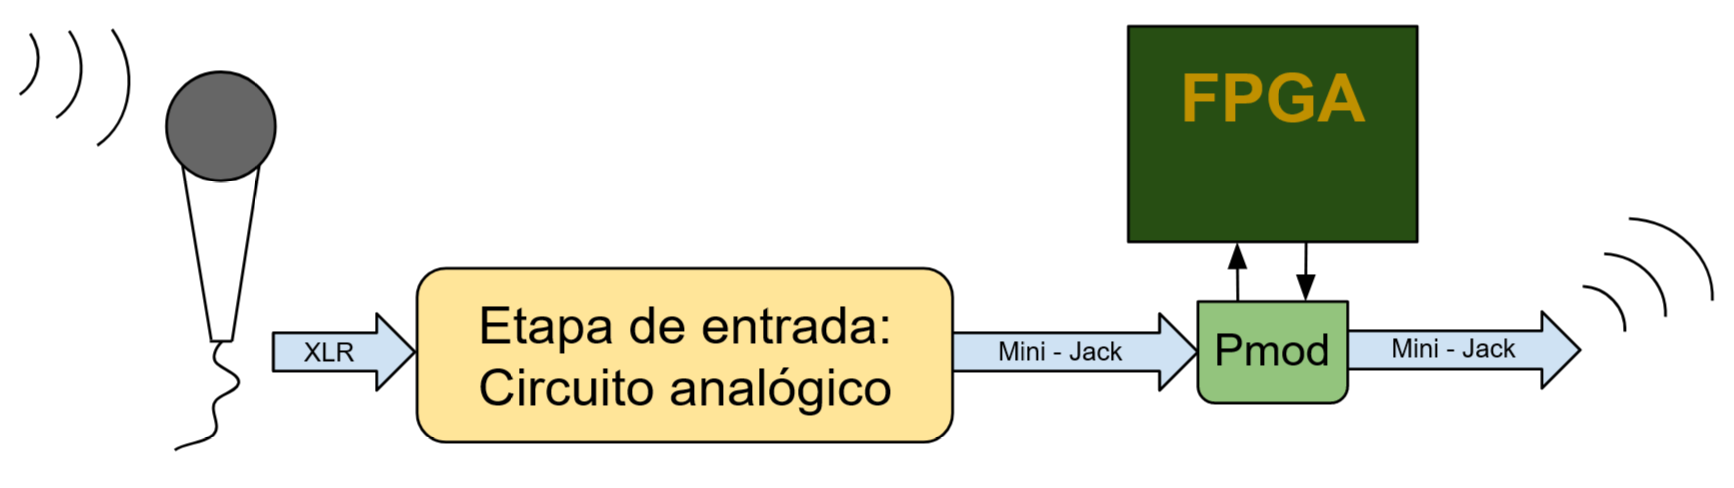
\includegraphics[width=14cm]{img/arquitectura.png}
\caption{\label{fig:arquitectura}Arquitectura general del proyecto}
\end{center}
\end{figure}


\section{Objetivos}
Para la realización de este proyecto de forma satisfactoria se ha establecido la consecución de una serie de objetivos que son los siguientes:
\begin{itemize}
\item Diseño de un sistema completo, a partir de una problemática definida previamente mediante el estudio del instrumento y las señales que produce.
\item Diseño teniendo en cuenta su futura implementación sobre la FPGA proporcionada.
\item Construcción de un prototipo para estudiar la problemática desde la práctica.
\item Afianzar, debido a todo esto, conocimientos adquiridos durante el Grado en diversos ámbitos como el procesamiento de señal y en concreto en la especialidad de Sistemas Electrónicos como la programación hardware, el montaje de un circuito analógico y la correcta comunicación entre todos los módulos.
\end{itemize}

\section{Metodología}
\begin{itemize}
\item En primer lugar se seleccionará el efecto que se quieren implementar, en este caso la octavación.
\item Como segundo paso, se estudiará la literatura existente y se probarán distintas soluciones algorítmicas empleando MATLAB.
\item Se procede al estudio y elección de la interfaces de entrada y salida. Selección de micrófono, ADC y DAC.
\item Una vez seleccionados los componentes, se desarrollo y verificaca el algoritmo seleccionado en VHDL empleando la herramienta Vivado de Xillinx.
\item Por último se montará un prototipo empleando la placa Nexys A7 de Digilent, el micrófono seleccionado anteriormente y el resto de dispositivos que fueran necesarios.
\item Durante todas las etapas se requiere de fases de testing y depuración.
\end{itemize}

\section{Resultados}
Transcurrido el tiempo de desarrollo del proyecto, que ha sido de un año natural, se han alcanzado varias metas aunque no se ha podido ver terminada una versión funcional del prototipo. 
\begin{itemize}
\item Tras el periodo de investigación, se ha seleccionado un algoritmo y se ha implementado en Matlab, permitiendo comprobar la viabilidad del mismo. 
\item Se ha montado un circuito analógico que funciona como etapa de entrada, amplificando la señal musical y adecuándola para su correcta interpretación por parte de la FPGA.
\item Aunque no se tiene una versión completa de la implementación VHDL del algoritmo elegido, si que se han diseñado la mayoría de las partes para poder estimar el funcionamiento final del sistema completo así como su arquitectura.
\end{itemize}

Dado que el proceso de realización del trabajo ha sido de un año natural, se han empleado muchas horas en cada una de las diferentes partes del mismo. Para comprender la magnitud del presente proyecto, se adjunta un desglose aproximado de las horas de trabajo en siguiente tabla: 
\newpage
\begin{table}[htb]
\centering
\begin{tabular}{l r}
%%%%%%%%%%%%%%%%%%%%%%%%%%%%%%%%%%%%%%%%%%%%%%%%%%%%%%%%%%%%%%%%%%%%%%%%%%%%%%%%%%%%%%%%%%%%%%%%%%%%%%%%
\multirow{2}{9cm}{\centering{\textbf{Algoritmo}}}                   &\multirow{2}{2cm}{\textbf{150h}}  \\
				                                                    &                                  \\
\hline
Investigación de los diferentes algoritmos                          &50h                               \\ 
Comparativa y evaluación de los mismos                              &70h                               \\
Pruebas en Matlab                                                   &30h                               \\
\hline 
\hline
\multirow{2}{9cm}{\centering{\textbf{Circuito analógico}}}          &\multirow{2}{2cm}{\textbf{20h}}   \\
				                                                    &                                  \\
\hline 
Fase de documentación y montaje del circuito elegido                &15h                               \\ 
Pruebas y medidas                                                   &5h                                \\
\hline 
\hline
\multirow{2}{9cm}{\centering{\textbf{Implementación}}}              &\multirow{2}{2cm}{\textbf{320h}}  \\
				                                                    &                                  \\
\hline
Caracterización y puesta en marcha de la entrada y salida de datos  &70h                               \\ 
Implementación del algoritmo de Matlab en VHDL usando Vivado        &100h                              \\
Depuración y pruebas                                                &150h                              \\
\hline 
\hline 
\multirow{2}{9cm}{\centering{\textbf{Otros}}}                       &\multirow{2}{2cm}{\textbf{50h}}   \\
				                                                    &                                  \\
\hline
Medidas y estimaciones sobre el prototipo final                     &10h                               \\ 
Realización de la memoria                                           &40h                               \\
\hline 
\hline
\multirow{2}{9cm}{\centering{\textbf{TOTAL}}}                       &\multirow{2}{2cm}{\textbf{540h}}  \\
				                                                    &                                  \\
\end{tabular}
%\caption{\label{tabla:tiempo}Relación de tiempo de trabajo destinado a cada ámbito.}
\end{table}

Esta aproximación se ha hecho en base a la fecha de los \emph{commit} de Github realizados asumiendo una media de 12 horas de trabajo a la semana durante las 45 semanas de trabajo en el proyecto.

\section{Consecución de los objetivos propuestos}

Una vez concluido el tiempo de trabajo, se pueden realizar las siguientes afirmaciones en referencia al grado de consecución de los objetivos previamente propuestos:

\begin{itemize}
\item Se ha diseñado el algoritmo para la octavación en su totalidad, atendiendo a criterios técnicos debidamente justificados en este documento.
\item Aunque no se ha llegado a implementar el sistema en su totalidad, sí que se ha trabajado en este aspecto en profundidad, permitiendo una estimación del funcionamiento de los módulos restantes que forman una idea general del funcionamiento del sistema completo.
\item El prototipo no es plenamente funcional pero sí que ha permitido la prueba y la puesta en práctica de los diferentes aspectos que se han diseñado e implementado.
\item Debido al trabajo de investigación realizado, se han adquirido nuevas ideas relacionadas con estos estos ámbitos que han sido puestas en práctica de forma crítica, asentando los conocimientos adquiridos durante el grado relacionados con estas materias.
\end{itemize}